\documentclass{article}
\usepackage{amsmath,amssymb,enumerate,bbm,calc,capt-of,ifthen}
\usepackage{graphicx}% Include figure files
\usepackage{epsfig}

\newtheorem{cntr}{do not use}
\newcommand{\tmop}[1]{\operatorname{#1}}
\newtheorem{definition}[cntr]{Definition}
\newtheorem{assumption}{Assumption}
\newcommand{\dueto}[1]{\textup{\textbf{(#1) }}}
\newtheorem{varremark}[cntr]{Remark}
\newenvironment{remark}{\begin{varremark}\em}{\em\end{varremark}}
\newcommand{\nin}{\not\in}
\newcommand{\tmem}[1]{{\em #1\/}}
\newtheorem{varnote}{Note}
\newenvironment{note}{\begin{varnote}\em}{\em\end{varnote}}
\newtheorem{proposition}[cntr]{Proposition}

\newenvironment{proof}{
  \noindent\textbf{Proof.}\ }{\hspace*{\fill}
  \begin{math}\Box\end{math}\medskip}

\newenvironment{proofof}[1]{
  \noindent\textbf{Proof of #1.}\ }{\hspace*{\fill}
  \begin{math}\Box\end{math}\medskip}

\newenvironment{proof*}[1]{
  \noindent\textbf{#1\ }}{\hspace*{\fill}
  \begin{math}\Box\end{math}\medskip}

\newtheorem{lemma}[cntr]{Lemma}
\newtheorem{corollary}[cntr]{Corollary}
\newtheorem{theorem}[cntr]{Theorem}
\newenvironment{enumeratenumeric}{\begin{enumerate}[1.]}{\end{enumerate}}
\newtheorem{algo}{Algorithm}

\numberwithin{cntr}{section}
\numberwithin{equation}{section}

\newcommand{\comment}[1]{}
%standard macros
\newcommand{\abs}[1]{\left| #1 \right|}%Absolute value
\newcommand{\absSmall}[1]{| #1 |}%Absolute value, small
\newcommand{\RR}[0]{{\mathbb{R}}}

%Handy macros

\newcommand{\vx}[0]{{\vec{x}}}
\newcommand{\vp}[0]{{\vec{p}}}
\newcommand{\vq}[0]{{\vec{q}}}
\newcommand{\vr}[0]{{\vec{r}}}
\newcommand{\vm}[0]{{\vec{m}}}
\newcommand{\vmb}[0]{{\vec{\mathbf{m}}}}
\newcommand{\vv}[0]{{\vec{v}}}

\newcommand{\oneto}[1]{{1 \ldots #1}}
\newcommand{\onetoN}[0]{{1 \ldots N}}
\newcommand{\Oto}[1]{{0 \ldots #1-1}}
\newcommand{\OtoN}{{0 \ldots N-1}}

\newcommand{\pointData}{{ \{ \vp_{i} \}_{i=\OtoN} }}
\newcommand{\tanData}{{ \{ \vm_{i} \}_{i=\OtoN} }}

\newcommand{\curveSet}{{ \{ \gamma_i(t) \}_{\Oto{M}}}}
\newcommand{\poly}{{\Gamma}}

\newcommand{\ball}[2]{ { B_{#1}(#2) } }
\newcommand{\allowed}[2]{ { A_{#1}(#2) } }

\newcommand{\curvemax}{{\kappa_{m}}}
\newcommand{\curvemaxi}{{\curvemax^{-1}}}

\newcommand{\curvesep}{{\delta}}

\newcommand{\pointNoise}{{\zeta}}
\newcommand{\tanNoise}{{\xi}}

\newcommand{\nallowed}[2]{ { A^{\pointNoise, \tanNoise}_{#1}(#2) } }

\begin{document}

\title{Reconstructing Curves from Points and Tangents}

\author{L. Greengard and C. Stucchio}

\maketitle

\begin{abstract}
  Reconstructing a finite set of curves from an unordered set of points sampled from the curves is a well studied topic. We ask the less studied question: can one do better if \emph{tangential} information is given as well?

  In this work, we answer this question, and show that if curves are separated from each other by a distance $\curvesep$, then the sampling rate need only be $O(\sqrt{\curvesep})$ for reconstruction. For the case of point data, $O(\curvesep)$ required.
\end{abstract}

\section{Introduction}

In this work, we consider the problem of reconstructing a $C^{1}$ \emph{figure} -- a family of curves $\curveSet$. The data we are given consists of an unorganized set of points $\pointData$, as well as \emph{unit} tangents to the points $\tanData$. Note that the tangents have no particular orientation; making the change $m_{i} \rightarrow -m_{i}$ destroys no information.

Our goal in this work is to construct an algorithm which reconstructs the polygonalization of the curve from this data. An example of a polygonalization is given in Figure \ref{fig:polygonalization}.

\begin{definition}
  \label{def:polygonalization}
  A polygonalization of a figure $\curveSet$ is a planar graph $(V,E)$ with the property that each vertex $p \in V$ is a point on some $\gamma_{i}(t)$, and each edge connects points which are adjacent samples of some curve $\gamma_{i}$.
\end{definition}

\begin{figure}
\setlength{\unitlength}{0.240900pt}
\ifx\plotpoint\undefined\newsavebox{\plotpoint}\fi
\sbox{\plotpoint}{\rule[-0.200pt]{0.400pt}{0.400pt}}%
\includegraphics[scale=0.5]{polygonalization_example.eps}

\caption{A figure and it's polygonalization, c.f. Definition \ref{def:polygonalization}. }
\label{fig:polygonalization}
\end{figure}

The topic of reconstructing figures solely from point data $\pointData$ has been the subject of considerable attention \cite{amenta98crust,amenta98new,dey99curve,hoppe92surface,amenta02simple, dey01reconstructing}. This is actually a more difficult problem, and only weaker results are possible. The main difficulty is the following; if the distance between two separate curves $\gamma_{i}$ and $\gamma_{j}$ is smaller than the sample spacing, then it is difficult to determine which points are associated to which curve. Thus, sample spacing must be $O(\curvesep)$, with $\curvesep$ the distance between different curves.

Tangential information makes this task easier; if two points are nearby (say $\vp_{1}$ and $\vp_{2}$), but $\pm \vm_{1}$ does not point (roughly) in the direction $\vp_{2}-\vp_{1}$, then $\vp_{1}$ and $\vp_{2}$ should not be connected. This fact allows us to reduce the sample spacing to $O(\curvesep^{1/2})$, rather than $O(\curvesep)$. This is to be expected; knowledge of a function and it's derivatives allows interpolation with quadratic accuracy.

We should mention at this point related work on \emph{Surfels} (short for \emph{Surface Elements}). A surfel is a point, together with information characterizing the tangent plane to a surface at that point (and perhaps other information such as texture). They have become somewhat popular in computer graphics recently, mainly for rendering objects characterized by point clouds \cite{882320,598521,344936,1018057,1103907,383300}.

In this work, we present an algorithm which allows us to reconstruct a curve from $\pointData$ and $\tanData$. We make two assumptions, under which the algorithm is provably correct.

\begin{assumption}
  \label{ass:curvature}
  We assume each curve $\gamma_{i}$ has bounded curvature:
  \begin{equation}
    \label{eq:curvatureAssumption}
    \forall i = \Oto{M}, ~ \frac{
      \abs{\gamma_{i,x}'(t) \gamma_{i,y}''(t) - \gamma_{i,y}'(t) \gamma_{i,x}''(t)}
    } {
      (\gamma_{i,x}'(t)^{2}+\gamma_{i,y}'(t)^{2})^{3/2}
    } \leq \curvemax
  \end{equation}
\end{assumption}

This assumption is necessary to prevent the curves from oscillating too much between samples.

\begin{assumption}
  \label{ass:separation}
  We assume the curves $\gamma_{i}$ and $\gamma_{j}$ are uniformly separated from each other, i.e.:
  \begin{subequations}
    \begin{equation}
      \label{eq:separationAssumption}
      \sup_{t,t'} \abs{ \gamma_{i}(t) - \gamma_{j}(t')} \geq \curvesep \textrm{~for~} i \neq j
    \end{equation}
    We also assume different areas of the same curve are separated
    from each other:
    \begin{equation}
      \label{eq:separationAssumptionSameCurve}
      \sup_{\abs{t-t'} > \curvemaxi\pi/2 } \abs{ \gamma_{i}(t) - \gamma_{i}(t')} \geq \curvesep
    \end{equation}
  \end{subequations}
  (assuming the curve $\gamma_{i}(t)$ proceeds with unit speed).
\end{assumption}

This assumption makes sure the curves do not come too close together for us to determine which points correspond to which curve (or which part of the same curve). This is illustrated in Figure \ref{fig:separationBetweenCurves}.

\begin{figure}
\setlength{\unitlength}{0.240900pt}
\ifx\plotpoint\undefined\newsavebox{\plotpoint}\fi
\sbox{\plotpoint}{\rule[-0.200pt]{0.400pt}{0.400pt}}%
\includegraphics[scale=0.5]{assumption_two.eps}

\caption{An illustration of Assumption \ref{ass:separation}. The black arrow illustrates \eqref{eq:separationAssumption}, while the red arrow illustrates \eqref{eq:separationAssumptionSameCurve}.}
\label{fig:separationBetweenCurves}
\end{figure}

\section{Geometry}
\subsection{Definition and notations}
Before we begin, we define some notation which we will use.

\begin{definition}
  \label{def:perp}
  For a vector $\vv$, let $\vv^{\perp}$ denote the vector $\vv$ rotated $\pi/2$ to the right.
\end{definition}

\begin{definition}
  \label{def:metric}
  Let $d(\vp,\vq)$ denote the usual Euclidean metric, $d(\vp,\vq) = \abs{\vp - \vq}$. Let $d_{\vm}(\vp,\vq)$ denote the distance in the $\vm$ direction between $\vp$ and $\vq$, i.e. $d_{\vm}(\vp,\vq) = \abs{ (\vp - \vq) \cdot \vm}$.
\end{definition}

\begin{definition}
  For a point $\vp$ and a curve $\gamma_{i}(t)$, we say that $\vp \in \gamma_{i}(t)$ if $\exists t, \gamma_{i}(t)=\vp$.
\end{definition}

As is normal for most interpolation theorems, we need an assumption on the variation of the curve, in this case the curvature.

\subsection{The Algorithm}

We assume there is a set of curves $\curveSet$, which we call the figure. Our goal is to construct a polygonalization of $\curveSet$ from data consisting of points $\pointData$ and tangent directions at the points, $\tanData$. Before we explain the algorithm that calculates the polygonalization, we prove a basic lemma which forms the foundation of our method.
\begin{lemma}
  \label{lem:forbiddenZone}
  For every $i \neq j$, if $\vp_{j} \in \ball{\curvemaxi}{\vp_{i} \pm \vm_{i}^{\perp} \curvemaxi}$, then $(\vp_{i},\vp_{j})$ is not an edge in $\poly$. Here, $\ball{r}{\vp}$ is the ball of radius $r$ about $\vp$.

  We refer to the set $\cup_{\pm} \ball{\curvemaxi}{\vp_{i} \pm \vm_{i}^{\perp} \curvemaxi}$ as the \emph{forbidden zone}; this region is illustrated in Fig. \ref{fig:forbiddenZone}.
\end{lemma}
\begin{figure}
\setlength{\unitlength}{0.240900pt}
\ifx\plotpoint\undefined\newsavebox{\plotpoint}\fi
\sbox{\plotpoint}{\rule[-0.200pt]{0.400pt}{0.400pt}}%
\includegraphics[scale=0.5]{forbidden_zone.eps}

\caption{The forbidden zones, as described in Lemma \ref{lem:forbiddenZone}. The pink is the forbidden zone, and the blue is the set of points a distance $\pi \curvemaxi/2$ away from $p_{i}$.}
\label{fig:forbiddenZone}
\end{figure}
\begin{proof}
  Suppose for simplicity that $\vp_{i}=(0,0)$ and $\vm_{i}=(1,0)$. Now, consider a line $\tau(t)$ of maximal curvature. The curve of maximal curvature, with $\tau_{y}'(t) > 0$ and proceeding at speed $\curvemaxi$ is $\tau^{+}(t)=(\curvemaxi \sin(t), \curvemaxi (1-\cos(t)))$, while the curve with $\tau_{y}'(t) < 0$ is $\tau^{-}(t)=(\curvemaxi \sin(t), \curvemaxi (\cos(t)-1))$.

Any other curve $\gamma(t)$ must lie between these curves (the blue and green curves in Fig \ref{lem:forbiddenZone}). Thus, it is confined to the blue region while it's arc length is less than $\curvemaxi \pi/2$. If $\gamma(t)$ connects $\vp_{i}$ to $\vp_{j}$, then it must do so after travelling a distance greater than $\curvemaxi \pi/2$.

\end{proof}

This shows that the extra information the tangents provides us can be used to exclude certain edges from the polygonalization; basically, all edges should point roughly in the direction of the tangent. This allows us to reject edges which would point in the wrong direction, yielding a more accurate polygonalization (c.f. Fig. \ref{fig:proximityVsTangentBased}).

\begin{figure}
\setlength{\unitlength}{0.240900pt}
\ifx\plotpoint\undefined\newsavebox{\plotpoint}\fi
\sbox{\plotpoint}{\rule[-0.200pt]{0.400pt}{0.400pt}}%
\includegraphics[scale=0.5]{tangents_good_for.eps}

\caption{A naive proximity-based reconstruction algorithm (shown), or even $\beta$-crust type algorithms, will add edges between different curves. Knowledge of the forbidden zone (indicated in pink) allows us to remove such edges.}
\label{fig:proximityVsTangentBased}
\end{figure}

\begin{definition}
  \label{def:AllowedRegion}
  Define the set $\allowed{\epsilon}{\vp}$ to be:
  \begin{equation}
    \label{eq:allowedRegion}
    \allowed{\epsilon}{\vp}=\ball{\epsilon}{\vp_{i}} \setminus \left[ \cup_{\pm} \ball{\curvemaxi}{\vp_{i} \pm \vm_{i}^{\perp} \curvemaxi} \right]
  \end{equation}
  That is, $\allowed{\epsilon}{\vp}$ is the ball of radius $\epsilon$ about $p$ excluding the forbidden zone.  We call this the \emph{allowed zone} or \emph{allowed region}.
\end{definition}
Any edge in the polygonalization starting at $\vp$, with length shorter than $\epsilon$, must connect to another point $\vq \in \allowed{\epsilon}{\vp}$.

We are now ready to describe the polygonalization algorithm.

\begin{algo}
  \label{algo:polygonalization}
  {\bf Polygonalization Algorithm }

  { \bf Input: }

  \begin{itemize}
  \item The maximal curvature, $\curvemax$.
  \item A parameter $\epsilon$ satisfying $\epsilon \curvemax < 2^{-1/2}$ and $2 \curvemax \epsilon^{2} < \curvesep$.
  \item The data $\pointData$ and $\tanData$. We assume that points adjacent on a given curve have a distance shorter than $\epsilon$ between them, i.e. the curve is $\epsilon$-sampled.
  \end{itemize}


  {\bf Algorithm: }

  \begin{enumerate}
  \item Compute the graph $G = (\pointData, E)$ with edge set:
    \begin{equation*}
      E = \{ (\vp_{i},\vp_{j}) : \vp_{i} \in \allowed{\epsilon}{\vp_{j}} \textrm{~and~} \vp_{j} \in \allowed{\epsilon}{\vp_{i}}\}
    \end{equation*}
  \item For each vertex $\vp_{i} \in \pointData$:
    \begin{enumerate}[a.]
    \item Compute the set of vertices
      \begin{equation*}
        R^{\pm}_{i} = \{ \vp_{j} : (\vp_{i}, \vp_{j}) \in E \textrm{~and~} \pm (\vp_{j}-\vp_{i}) \cdot \vm_{i} > 0 \}
      \end{equation*}
    \item Find the nearest tangential neighbors, i.e.
      \begin{equation*}
        \vr^{\pm}_{i} = \textrm{argmin}_{\vq \in R^{\pm}_{i}} d_{\vm_{i}}(\vq, \vp_{i})
      \end{equation*}
    \end{enumerate}
  \item Output the graph $\Gamma = ( \pointData, E')$ with
    \begin{equation*}
      E' = \{ (\vp_{i}, \vr^{+}_{i}) \} \cup \{ (\vp_{i}, \vr^{-}_{i}) \}
    \end{equation*}
    This graph is the polygonalization of $\curveSet$.
  \end{enumerate}

\end{algo}

We also have the following result, which guarantees the correctness of Algorithm \ref{algo:polygonalization}.

\begin{theorem}
  \label{thm:proofOfAlgo}
  Suppose that:
  \begin{subequations}
    \label{eq:separationCondition}
    \begin{equation}
      \label{eq:constraintOnSeparationSampling}
      \curvesep > 2\curvemax \epsilon^{2}
    \end{equation}
    where $\curvesep$ is as in Assumption \ref{ass:separation} and also
    \begin{equation}
      \label{eq:constraintOnkmaxEpsilon}
      \epsilon < \frac{1}{ \curvemax \sqrt{2}}
    \end{equation}
  \end{subequations}
  Suppose also that the distance between adjacent samples in the polygonalization is bounded by $\epsilon$, i.e. the curve is $\epsilon$-sampled. Then graph $\Gamma$ returned by Algorithm \ref{algo:polygonalization} is the polygonalization of $\curveSet$.
\end{theorem}

We prove this shortly.

\begin{remark}
  As presented, the complexity of Algorithm \ref{algo:polygonalization} is $O(N^{2})$, due to both step 1 and step 2. (Step 2 can be slow if $O(N)$ points are within the allowed region of some particular point). The complexity can be reduced to $O(N \log N)$; this is discussed in Appendix \ref{sec:quadTreeSection}.
\end{remark}

\subsection{Proof of Theorem \ref{thm:proofOfAlgo}}

\begin{lemma}
  \label{lem:separationAllowedRegions}
  Let $i \neq j$ and let Assumption \ref{ass:separation} hold. Then for all $t, t'$, if \eqref{eq:separationCondition} holds, then
  \begin{equation}
    \label{eq:connectionsBetweenDifferentCurvesNotAllowed}
    \gamma_{j}(t')  \nin  \allowed{\epsilon}{\gamma_{i}(t)}.
  \end{equation}
  Similarly, if $i=j$ and $\abs{t-t'} \geq \curvemax^{-1} \pi/2$, then \eqref{eq:connectionsBetweenDifferentCurvesNotAllowed} holds.
\end{lemma}
\begin{proof}
  Fix $t$, and define $\vp=\gamma_{i}(t)$ and $\vm=\gamma_{i}'(t) / \abs{\gamma_{i}'(t)}$. Define $L$ to be the line segment $L= \{ \vp+\vm \curvemaxi \sin(\theta) : \theta \in [-\arcsin(\epsilon \curvemax),\arcsin(\epsilon \curvemax)] \}$. The boundaries of $\allowed{\epsilon}{\vp}$ are given by
\begin{equation*}
  \vp + \vm \curvemaxi \sin(\theta) \pm \vm^{\perp} \curvemaxi (1-\cos(\theta)).
\end{equation*}
Now, for any $\vq \in \gamma_{i} $ and $\vq \in \allowed{\epsilon}{\vp}$, the distance between $\vq$ and $L$ is the normal distance to $L$. This distance is bounded by:
\begin{multline}
  \label{eq:1}
  d(\vq,L) \leq
  \sup_{\theta} \curvemaxi \abs{(1-\cos(\theta)) }\\
  \leq
  \sup_{\theta} \curvemaxi 2 \sin^{2}(\theta/2) =
  2\curvemaxi \sin^{2}( \arcsin(\epsilon \curvemax)/2)
\end{multline}
The intermediate value theorem implies $\arcsin( x) \leq \arcsin'(\zeta) x=(1-\zeta^{2})^{-1/2} x$ for some $\zeta \in [0,x]$; since $\epsilon \curvemax < 2^{-1/2}$ (by \eqref{eq:constraintOnkmaxEpsilon}), we find that:
\begin{equation*}
  \arcsin(\epsilon \curvemax) \leq (1-(2^{-1/2})^{2})^{-1/2} \curvemax \epsilon = \sqrt{2} \curvemax \epsilon
\end{equation*}
Substituting this into \eqref{eq:1} yields:
\begin{equation}
  \eqref{eq:1} \leq  2 \curvemaxi \sin^{2}( \sqrt{2} \curvemax \epsilon/2) \leq \curvemax \epsilon^{2}
\end{equation}

Thus, the \emph{normal} distance between any point in $\allowed{\epsilon}{\vp}$ and $L$ is $O(\curvemax \epsilon^{2})$.

If $\gamma_{j}(t') \nin L+\vm^{\perp} \RR$, then clearly $\gamma_{j}(t') \nin \allowed{\epsilon}{\gamma_{i}(t)}$ so we assume $\gamma_{j}(t') \in L+\vm^{\perp} \RR$. In this case, $\gamma_{j}(t') = \vp + \vm \curvemaxi \sin(\theta_{0}) + \vm^\perp z$, with $z \in \RR$ the normal (relative to $L$) distance to $L$.

By the second triangle inequality,
\begin{equation*}
  d_{\vm^{\perp}}(\gamma_{j}(t'), L) \geq \abs{d_{\vm^{\perp}}(\gamma_{j}, \gamma_{i}) -  d_{\vm^{\perp}}(\gamma_{i}, L)}
  \geq \delta - \curvemax \epsilon^{2} > \curvemax \epsilon^{2}
\end{equation*}
But this implies that $d(\gamma_{j}(t'), L) \geq d_{\vm^{\perp}}(\gamma_{j}(t'), L) \geq \curvemax \epsilon^{2}$, and thus $\gamma_{j}(t') \nin \allowed{\epsilon}{\vp}$.

The proof when $i=j$ is identical.
\end{proof}

This result shows that the graph $G$, computed in Step 1 of Algorithm \ref{algo:polygonalization}, separates different $\gamma_{i}$ and $\gamma_{j}$ from each other, as well as different parts of the same curve. Thus, after Step 1, we are left with a graph $G$ having edges only between points $\vp_{i}$ and $\vp_{j}$ which are on the same curve $\gamma_{k}$, and which have are separated in $\gamma_{k}$ by an arc length no more than $\curvemaxi \pi/2$.

We now show that $G$ is a superset of the polygonalization.

\begin{proposition}
  \label{prop:polyIncludesNeighboringPoints}
  Suppose the point data $\pointData$ is $\epsilon$-sampled, i.e. if two points $\vp_{i}$ and $\vp_{j}$ are adjacent on the curve $\gamma_{k}$, then the \emph{arc length} between $\vp_{i}$ and $\vp_{j}$ is bounded by $\epsilon$. Then $G$ contains the polygonalization of $\curveSet$.
\end{proposition}
\begin{proof}
  If the distance between adjacent points $\vp_{i}$ and $\vp_{j}$ is at most $\epsilon$, then $\vp_{j} \in \ball{\epsilon}{\vp_{i}}$. Since the segment of $\gamma_{k}$ between $\vp_{i}$ and $\vp_{j}$ has arc length less than $\epsilon$, $\vp_{j}$ is not in the forbidden zone of $\vp_{i}$ (by the same argument as in Lemma \ref{lem:forbiddenZone}. Thus, $\vp_{j} \in \allowed{\epsilon}{\vp_{i}}$ (and vice versa), and $(\vp_{i},\vp_{j})$ is an edge in $G$.
\end{proof}

We have now shown that $G$ separates distinct curves, and that $G$ contains the polygonalization of $\curveSet$. It remains to show that $\Gamma$ is the polygonalization.

\begin{lemma}
  \label{lem:localGraphParameterization}
  A curve $\gamma_{i}(t)$ satisfying \eqref{eq:curvatureAssumption} admits the local parameterization
  \begin{equation}
    \label{eq:localGraphParameterization}
    \gamma_{i}(t) = \gamma(t_{0}) + (t-t_{0})\gamma'(t_{0}) + w(t) \gamma'^{\perp}(t_{0})
  \end{equation}
  where $w'(t_{0})=0$. The parameterization is valid for $\abs{t-t_{0}} < \curvemaxi$.
\end{lemma}

\begin{proof}
  Taylor's theorem shows the parameterization to be valid on an arbitrarily small ball. All we need to do is show that this parameterization is valid on a region of size $\curvemaxi$.

  The parameterization breaks down when $w'(t)$ blows up, so we need to show that this does not happen before $t=\epsilon$. Plugging this parameterization into the curvature bound \eqref{eq:curvatureAssumption} yields:
  \begin{equation*}
    \frac{ \abs{w''(t)} }{(1+w'(t)^{2})^{3/2}} \leq \curvemax
  \end{equation*}
  Assuming $w''(t)$ is positive, this is a first order nonlinear differential inequality for $w'(t)$. We can integrate both sides (using the hyperbolic trig substitution $w(t)=\sinh(\theta)$ for the left side) to obtain:
  \begin{equation}
    \label{eq:2}
    \frac{w'(t)}{\sqrt{1+w'(t)^{2}}} \leq \curvemax t
  \end{equation}
  Define $f(z)=z/\sqrt{1+z^{2}}$, then $f^{-1}(z)$ is singular only at $z=\pm 1$, and is regular before that. Solving \eqref{eq:2} for $w'(t)$ shows that:
  \begin{equation*}
    w'(t) \leq f^{-1}(\curvemax t)
  \end{equation*}
  implying that $w'(t)$ is finite for $\curvemax t < 1$, or $t < \curvemaxi$.
\end{proof}

\begin{lemma}
  \label{lem:closestTangentPointInAllowedRegionIsCorrect}
  Fix a point $\vp_{i}=\vp \in \pointData$. Choose a tangent vector $\vm_{0}$ and fix an orientation. Consider the set of points $\vp_{j}$ such that $(\vp, \vp_{j})$ is an edge in $G$ and $(\vp_{j} - \vp) \cdot \vm_{0} > 0$. Suppose also that $\epsilon$ satisfies \eqref{eq:constraintOnkmaxEpsilon}.

  Then only edge in the polygonalization of $\gamma$ is the edge for which $(\vp_{j} - \vp) \cdot \vm_{0}$ is minimal.
\end{lemma}

\begin{remark}
  The minimal edge is the edge $\vr^{+}_{0}$ as computed in Step (2b) of Algorithm \ref{algo:polygonalization}.
\end{remark}

\begin{proof}
  By Lemma \ref{lem:localGraphParameterization}, the curve $\gamma(t)$ can be locally parameterized as a graph near $\vp$, i.e. \eqref{eq:localGraphParameterization}. This is valid up to a distance $\curvemaxi$; by \eqref{eq:constraintOnkmaxEpsilon}, it is valid for all points in the graph $G$ connected to $\vp$.

The adjacent points on the graph are the ones for which $\abs{t-t_{0}}$ is minimal. Note that $\vm_{0} \cdot (\vp_{j} - \vp) = t$ (simply plug in \eqref{eq:localGraphParameterization}); thus, minimizing $\vm_{0} \cdot (\vp_{j} - \vp)$ selects the adjacent point on the graph.
\end{proof}

Thus, we have shown that the graph $\Gamma$, as computed by Algorithm \ref{algo:polygonalization}, is the polygonalization of $\curveSet$.

\begin{figure}
\setlength{\unitlength}{0.240900pt}
\ifx\plotpoint\undefined\newsavebox{\plotpoint}\fi
\sbox{\plotpoint}{\rule[-0.200pt]{0.400pt}{0.400pt}}%
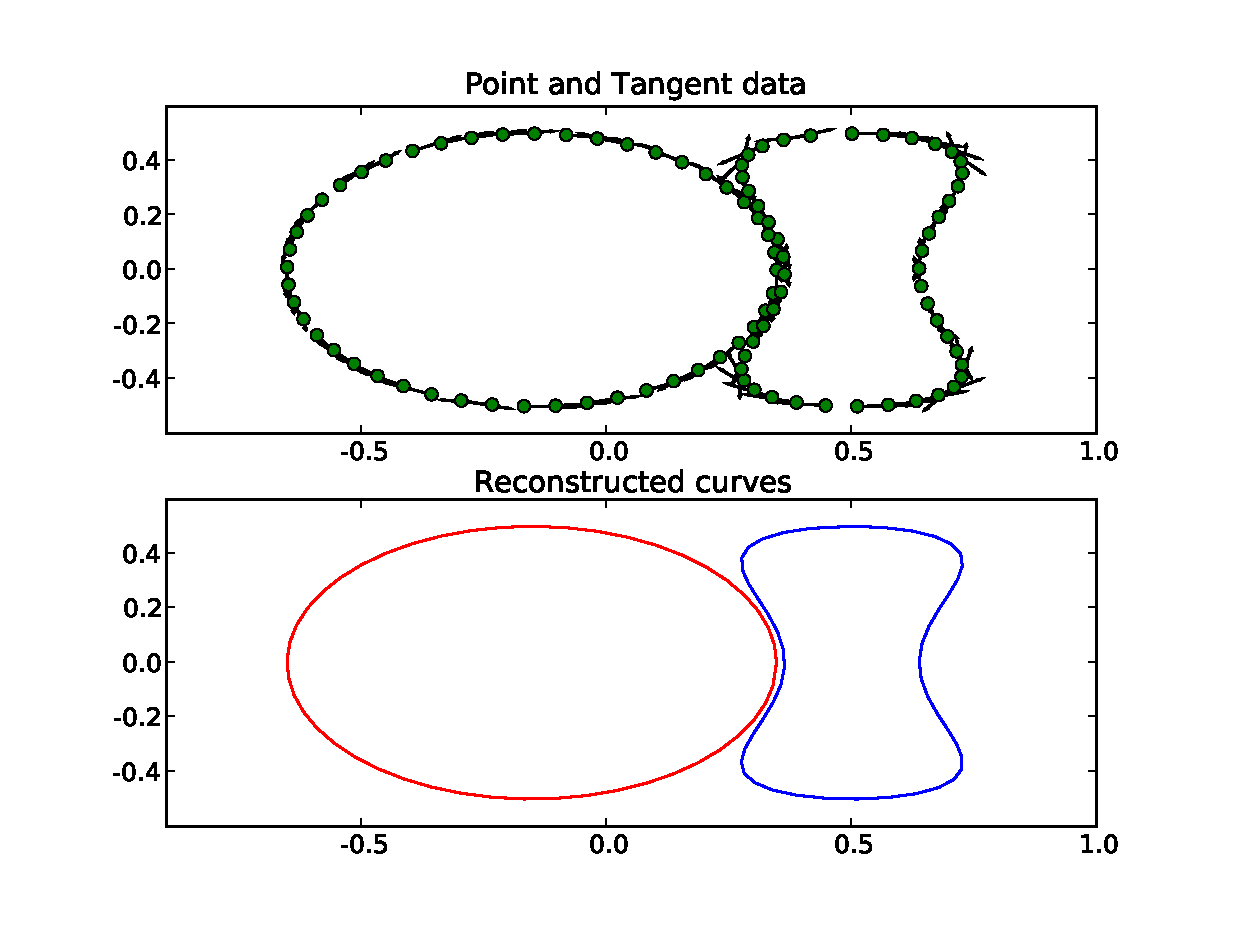
\includegraphics[scale=0.5]{example1.eps}

\caption{Some unordered points/tangents, and the curves reconstructed from them. In this case, $\epsilon=0.065$, $\curvemax=3$ and $\delta=0.015$.}
\label{fig:basicExample}
\end{figure}

\section{Noisy Data}

In real life, one rarely has perfect data. For this reason, it is important to consider the case of noisy data. Toward that end, we consider the polygonalization problem, but with the point data perturbed by noise smaller than $\pointNoise$ and tangent data perturbed by noise smaller than $\tanNoise$.

By this we mean the following; to each point $\vp_{i} \in \pointData$, there exists a point $\vp_{i}' = \gamma_{k_{i}}(t_{i})$ such that $\abs{\vp_{i}-\vp_{i}'} \leq \pointNoise$. Similarly, the unit tangent vector $\vm_{i}$ differs from the true tangent $\vm_{i}' = \gamma_{k_{i}}'(t_{i})$ by an angle at most $\tanNoise$. By a a polygonalization of the noisy data, we mean that $(\vp_{i},\vp_{j})$ is an edge in the noisy polygonalization if $(\vp_{i}',\vp_{j}')$ is an edge in the non-noisy polygonalization. In what follows, $\vp_{j}$ refers to a given (noisy) point, while $\vp_{j}'$ refers to the corresponding true point (and similarly for tangents).

Of course, the noise introduces a lower limit on the features we can resolve. Obviously, the curves must be separated by a distance at least $\pointNoise$, to prevent noise from actually moving a sample from one curve to another. More seriously, noise in the tangent data introduces uncertainty which forces us to increase the sampling rate; in particular, we require $O(\epsilon \tanNoise + \epsilon^{2}) < \curvesep$.

The main idea in extending Algorithm \ref{algo:polygonalization} to the noisy case is to expand the allowed regions to encompass all possible points and tangents. Of course, this imposes new constraints on the separation between curves.

We also require a \emph{minimal} sampling rate in order to ensure that the order of points on the curve is not affected by noise.

\begin{assumption}
  \label{ass:minSamplingRateNoisy}
  We assume that adjacent points $\vp_{i}$ and $\vp_{j}$ on the curve $\gamma_{k}(t)$ are separated by a distance greater than $2\pointNoise + ?$.
\end{assumption}

To extend to the noisy case, we must expand the allowed region to account for our uncertainty concerning the actual location of points.

\begin{definition}
  \label{def:AllowedRegionNoisy}
  Define the \emph{noisy allowed region} $\nallowed{\epsilon}{\vp}$ to be:
  \begin{equation}
    \label{eq:allowedRegionNoisy}
    \nallowed{\epsilon}{\vp}= \bigcup_{
      \substack{
        \abs{\vp'-\vp_{i}} < \pointNoise\\
        \arccos(\vm_{i} \cdot \vm') < \tanNoise
      }
    }
    \left(
      \ball{\epsilon}{\vp'} \setminus \left[ \cup_{\pm} \ball{\curvemaxi}{\vp' \pm \vm'^{\perp} \curvemaxi} \right]
    \right)
  \end{equation}
  That is, $\nallowed{\epsilon}{\vp}$ is the union of all the allowed regions of points/tangents near $(\vp, \vm)$.
\end{definition}

\begin{algo}
  \label{algo:polygonalizationNoisy}
  {\bf Noisy Polygonalization Algorithm }

  { \bf Input: }

  \begin{itemize}
  \item The maximal curvature, $\curvemax$, and noise amplitudes $\pointNoise, \tanNoise$.
  \item A parameter $\epsilon$ satisfying $\epsilon \curvemax < 2^{-1/2}$ and $2 \curvemax \epsilon^{2} < \curvesep$. //FIX THIS
  \item The data $\pointData$ and $\tanData$. We assume that points adjacent on a given curve have a distance shorter than $\epsilon$ between them, i.e. the curve is $\epsilon$-sampled.
  \end{itemize}


  {\bf Algorithm: }

  \begin{enumerate}
  \item Compute the graph $G = (\pointData, E)$ with edge set:
    \begin{equation}
      \label{eq:noisyConditionForCheckingIfEdgeConnectionIsPlausible}
      E = \{ (\vp_{i},\vp_{j}) : \ball{\pointNoise}{\vp_{i}} \cap \nallowed{\epsilon}{\vp_{j}} \neq \emptyset  \textrm{~and~} \ball{\pointNoise}{\vp_{j}} \cap \nallowed{\epsilon}{\vp_{i}} \neq \emptyset \}
    \end{equation}
  \item For each vertex $\vp_{i} \in \pointData$:
    \begin{enumerate}[a.]
    \item Compute the set of vertices
      \begin{equation*}
        R^{\pm}_{i} = \{ \vp_{j} : (\vp_{i}, \vp_{j}) \in E \textrm{~and~} \pm (\vp_{j}-\vp_{i}) \cdot \vm_{i} > 0 \}
      \end{equation*}
    \item Find the nearest tangential neighbors, i.e.
      \begin{equation*}
        \vr^{\pm}_{i} = \textrm{argmin}_{\vq \in R^{\pm}_{i}} d_{\vm_{i}}(\vq, \vp_{i})
      \end{equation*}
    \end{enumerate}
  \item Output the graph $\Gamma = ( \pointData, E')$ with
    \begin{equation*}
      E' = \{ (\vp_{i}, \vr^{+}_{i}) \} \cup \{ (\vp_{i}, \vr^{-}_{i}) \}
    \end{equation*}
    This graph is the polygonalization of $\curveSet$.
  \end{enumerate}

\end{algo}


The next result parallels Proposition \ref{prop:polyIncludesNeighboringPoints}, and shows that the noisy allowed region contains nearby points on the polygonalization.

//NEED CALCULATIONS SHOWING NECESSARY DISTANCE BETWEEN CURVES, ANALGOUS TO LEMMA \ref{lem:separationAllowedRegions}//

\begin{proposition}
  Suppose the figure is sampled at a rate satisfying \eqref{eq:constraintOnkmaxEpsilon}. Then $G$ contains the polygonalization of the figure.
\end{proposition}

\begin{proof}
  The point $\vp_{i}$ and tangent $\vm_{i}$ are close to some point $\vp_{i}', \vm_{i}'$ on the figure $\curveSet$; in particular, $\abs{\vp_{i} - \vp_{i}'} \leq \pointNoise$ and $\arccos(\vm_{i} \cdot \vm_{i}') < \tanNoise$ . Similarly, there is a point $\vp_{j}'$ on the figure a distance no more than $\pointNoise$ away from $\vp_{j}$. By Proposition \ref{prop:polyIncludesNeighboringPoints}, $\vp_{j}' \in \allowed{\epsilon}{\vp_{i}'}$. Since $\vp_{j}' \in \ball{\pointNoise}{\vp_{j}}$ and $\vp_{j}' \in \allowed{\epsilon}{\vp_{i}'} \subset \nallowed{\epsilon}{\vp_{i}}$, we find that $\vp_{j}' \in \ball{\pointNoise}{\vp_{j}} \cap \nallowed{\epsilon}{\vp_{i}} \neq \emptyset$. Repeating this argument with $i$ and $j$ interchanged shows that \eqref{eq:noisyConditionForCheckingIfEdgeConnectionIsPlausible} holds, and $(\vp_{i}, \vp_{j})$ is an edge of $G$.
\end{proof}

\begin{proposition}
  \label{lem:noisyClosestTangentPointInAllowedRegionIsCorrect}
  Fix a point $\vp_{i}=\vp \in \pointData$, and suppose that Assumption \ref{ass:minSamplingRateNoisy} holds. Choose a tangent vector $\vm_{0}$ and fix an orientation. Consider the set of points $\vp_{j}$ such that $(\vp, \vp_{j})$ is an edge in $G$ and $(\vp_{j} - \vp) \cdot \vm_{0} > 0$. Suppose also that $\epsilon$ satisfies \eqref{eq:constraintOnkmaxEpsilon}.

  Then only edge in the polygonalization of $\gamma$ is the edge for which $(\vp_{j} - \vp) \cdot \vm_{0}$ is minimal.
\end{proposition}

\begin{proof}
  The idea of the proof follows that of Lemma \ref{lem:closestTangentPointInAllowedRegionIsCorrect} closely, but we must adjust for our uncertainty as to the point and tangent.

  The curve itself has the parameterization $\gamma(t) = \vp' + \vm' t + \vm'^{\perp} w(t)$, by Lemma \ref{lem:localGraphParameterization}, and this is valid for $\abs{t} < \curvemaxi$. However, we do not know $\vp'$ and $\vm'$, only $\vp$ and $\vm$. We wish to find the point $\vp_{j}$ for which $\vm' \cdot (\vp_{j}' - \vp')$ is minimal.

  Note that:
  \begin{multline*}
    \vm \cdot (\vp - \vp_{j}) = \vm \cdot (\vp' - \vp_{j}') + \vm \cdot ([\vp - \vp'] - [\vp_{j} - \vp_{j}']) \\
    = \vm' \cdot (\vp' - \vp_{j}') + (\vm - \vm') \cdot (\vp' - \vp_{j}')  + \vm \cdot ([\vp - \vp'] - [\vp_{j} - \vp_{j}'])
  \end{multline*}
  Or:
  \begin{multline*}
    \abs{
      \vm \cdot (\vp - \vp_{j}) - \vm' \cdot (\vp' - \vp_{j}')
      } \\
      \leq \abs{(\vm - \vm') \cdot (\vp' - \vp_{j}')}  + \abs{ \vm \cdot ([\vp - \vp'] - [\vp_{j} - \vp_{j}']) } \\
      \leq \sqrt{\sin^{2}(\tanNoise) + (1-\cos(\tanNoise) )^{2}}\abs{\vp' - \vp_{j}'} + 2 \pointNoise \leq 2 \tanNoise \abs{\vp' - \vp_{j}'} + 2\pointNoise
  \end{multline*}
//FINISH THIS UP, MIN SAMPLING MEANS DISTANCE BETWEEN $\vp_{j}$ and $\vp_{k}$

\end{proof}


//FINISH THIS SECTION//

\section{Examples}

\subsection{Hiding behind tree branches}

//SOUHEIL MENTIONED THIS EXAMPLE. NEED REFERENCES.//

Anyone who has played the game ``Hide and Seek'' knows that playing the role of seeker is more difficult in the summer than in the fall. This is because in the summer, trees have full foliage, which can completely block view of the hider. In the fall, this strategy no longer works, since trees lose their leaves. However, if the seeker is a robot, the strategy may still work; the bare branches can make it difficult to recognize the hider.

As a model of this problem\footnote{In particular, we are attempting to model the image after applying directional edge detectors to it, thus resulting in a set of points and tangents.}, we constructed a figure, and obscured it by placing it behind a sequence of lines. Algorithm \ref{algo:polygonalization} succesfully reconstructs the figure (the red oval), as well as properly connecting points on the horizontal and vertical ``branches''. The result is shown in Figure \ref{fig:obscuredExample}. Note that the branches are not connected to the oval (or each other).

\begin{figure}
\setlength{\unitlength}{0.240900pt}
\ifx\plotpoint\undefined\newsavebox{\plotpoint}\fi
\sbox{\plotpoint}{\rule[-0.200pt]{0.400pt}{0.400pt}}%
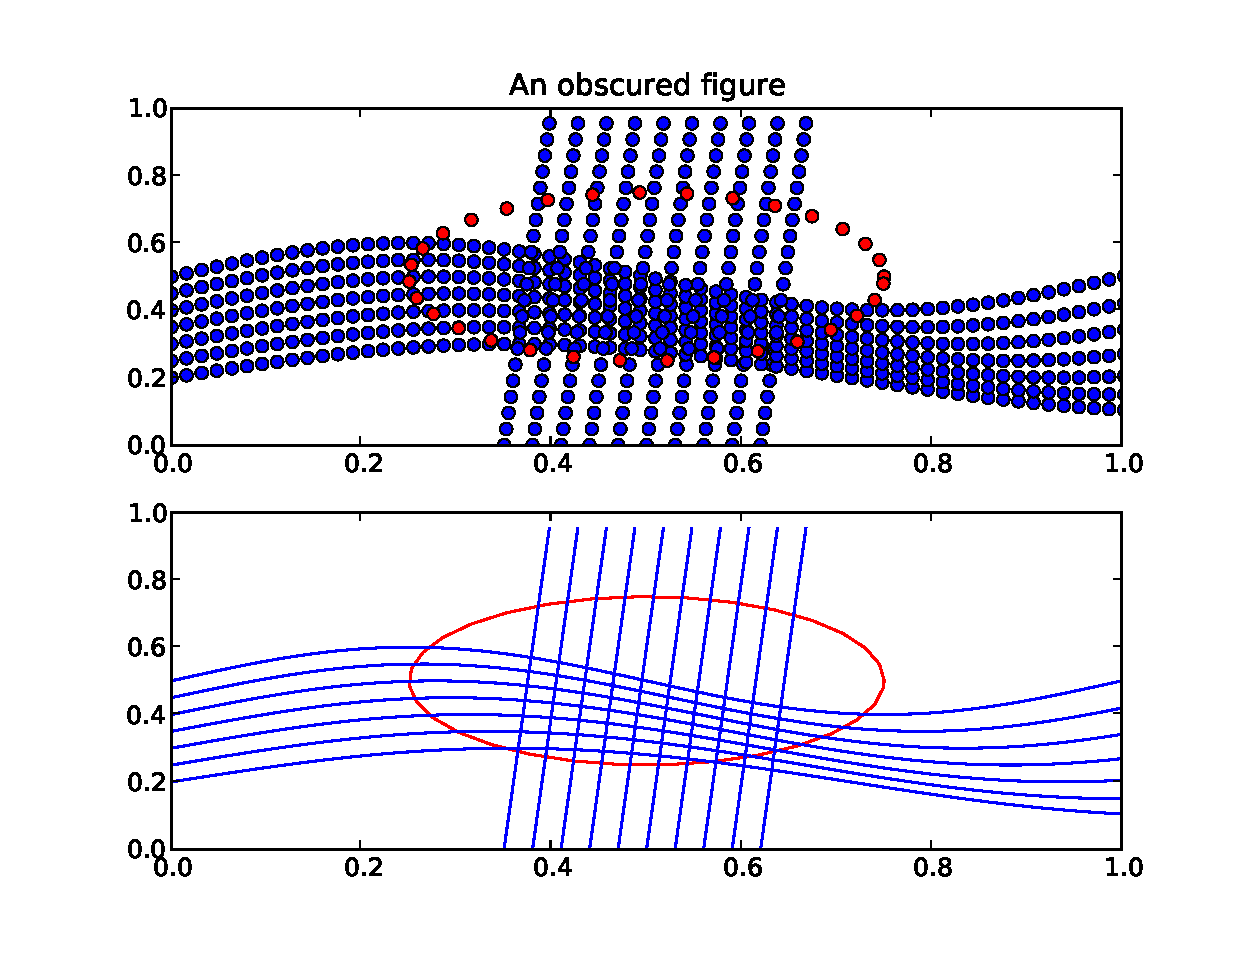
\includegraphics[scale=0.5]{obscured_figure.eps}

\caption{A figure which is partially obscured. Algorithm \ref{algo:polygonalization} correctly computes it's polygonalization, and distinguishes it from the curves in front of it. To avoid visual clutter, the tangents are not displayed in this figure.}
\label{fig:obscuredExample}
\end{figure}

\subsection{Filtering spurious points}

The method provided here is relatively robust with regard to the addition of spurious random data points. This is because spurious data points are highly unlikely to be connected to any other points in the polygonalization graph.

This occurs for two primary reasons. First, for an incorrect data point to be connected to part of the polygonalization at all, it would need to be located in $\allowed{\epsilon}{\vp}$ for some $\vp$. This is a region of length $O(\epsilon)$ and width $O(\epsilon^{2})$. There are approximately $L = \sum_{j} \textrm{arclength}(\gamma_{j})$ such points, for a total volume of $\epsilon^{2} L$. Thus, the probability that a spurious point is in \emph{some} allowed region is roughly $O(L \epsilon^{2})$.

The second reason is that even if a spurious point is in some allowed region, it is unlikely to point in the correct direction. If an erroneous point $\vq$ is inside $\allowed{\epsilon}{\vp}$, it is still not likely that $\vp \in \allowed{\epsilon}{\vq}$; this follows because the tangent at $\vq$ must point in the direction of $\vp$ (with error proportional to $\epsilon^{2}$, the angular width of $\allowed{\epsilon}{\vq}$). Thus, the probability that the tangent at $\vq$ points towards $\vp$ is $O(\epsilon^{2}/2\pi)$.

Based on these arguments, the probability that any \emph{randomly chosen} spurious point $\vq$ is connected to any other point in the polygonalization is $O(L \epsilon^{4})$.

\begin{figure}
\setlength{\unitlength}{0.240900pt}
\ifx\plotpoint\undefined\newsavebox{\plotpoint}\fi
\sbox{\plotpoint}{\rule[-0.200pt]{0.400pt}{0.400pt}}%
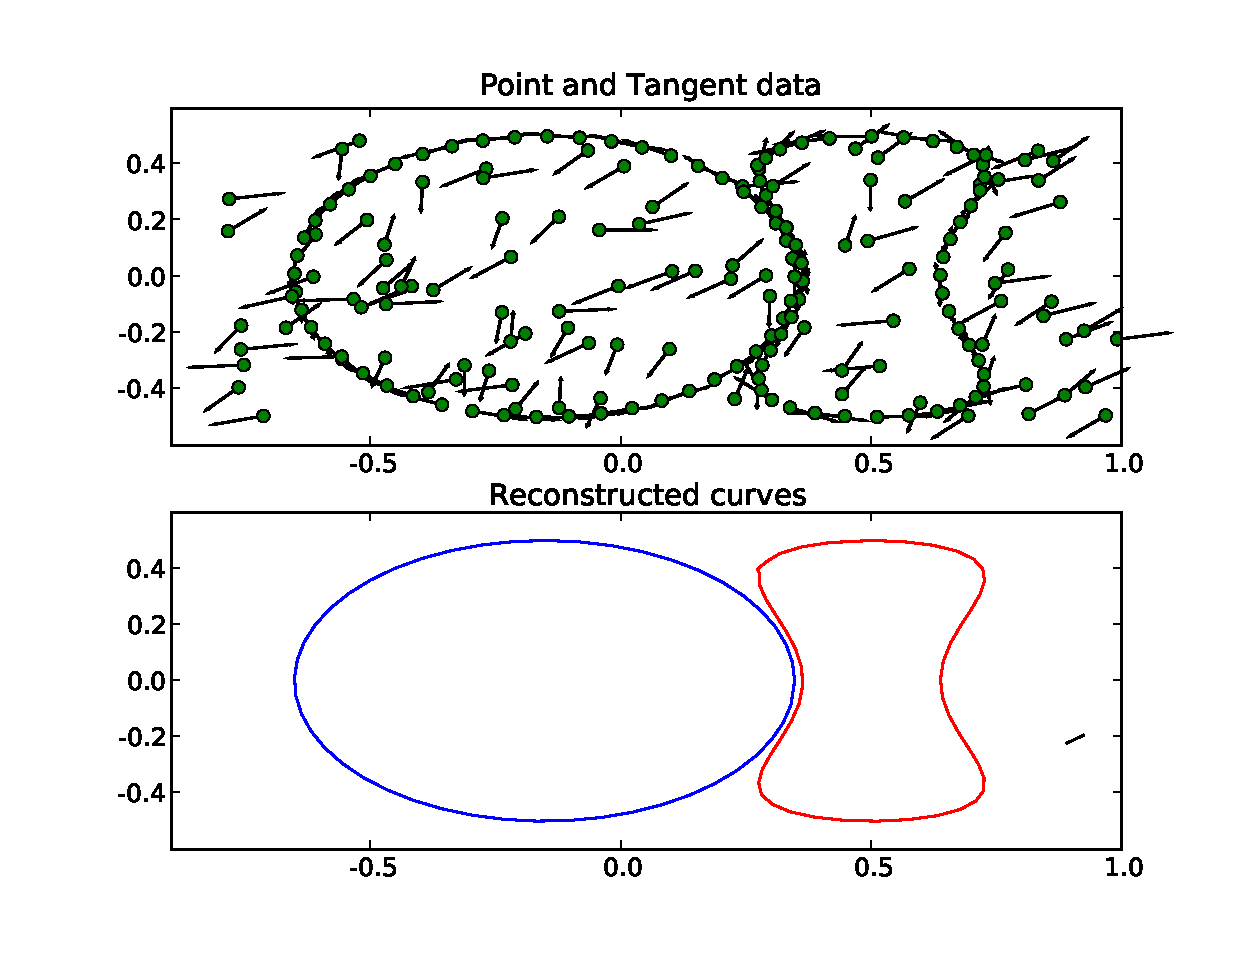
\includegraphics[scale=0.5]{noisy_example.eps}

\caption{The same example as in Figure \ref{fig:basicExample}, but with 100 additional points (for a total of $196$), placed randomly. }
\label{fig:noisyExample}
\end{figure}

\subsubsection{Noise Removal by Connecting the Dots}

The aforementioned criteria suggest that our ``connect the dots'' algorithm has excellent potential for noise removal. It suggests that if we remove points which do not have edges pointing towards other edges, then with high probability we are removing spurious edges.

In fact, this is born out in practice. By running Algorithm \ref{algo:polygonalization} on a figure consisting of $96$ true points, and $100$ randomly placed incorrect points, a nearly correct polygonalization is calculated; this is shown in Figure \ref{fig:noisyExample}. The original curve is reconstructed with an error at only one point (the top left corner of the red line).

Of course, if enough incorrect points are present, eventually some points will be connected by Algorithm \ref{algo:polygonalization}. This can be seen in Figure \ref{fig:noisyExample}: the black line near $(0.9, -0.2)$ is an edge between two incorrect points. However, spurious edge formations such as this are small in number, and do not usually look like part of the figure.

One hint that an edge is incorrect is if it points to a leaf. That is, consider a set of vertices $\vp_{0}, \vp_{1}, \ldots, \vp_{n}$ as well as $\vq$. Suppose, after approximately computing the polygonalization, one finds that the graph contains edges $e_{0} = (\vp_{0}, \vp_{1}), e_{1} = (\vp_{1}, \vp_{2}), \ldots, e_{n-1} = (\vp_{n-1}, \vp_{n})$ and $e_{n} = (\vp_{n/2}, \vq)$. The vertex $\vq$ is a leaf, i.e. it is reachable by only one edge. A polygonalization should not have leaves, suggesting that the edge $e_{n}$ should not be present. This suggests that by filtering leaves, we can remove primarily noise while leaving the signal undamaged.

An additional problem with noisy data is that sometimes, an incorrect point will be present, in the allowed region of a legitimate point, and closer to the legitimate point than the adjacent points along the curve. This will prevent the correct edge from being added. This can be remedied by adding not only $\vr_{i}^{\pm}$ at Step 3 of the algorithm, but also points for which $d_{\vm^{\perp}}(\vp_{i})$who's distance to $\vp_{i}$ is not much longer than the distance between $\vp_{i}$ and $\vr_{i}^{\pm}$. With some luck, this procedure combined with filtering out leaves will approximately reconstruct the correct figure.

Thus, we arrive at are noisy polygonalization algorithm.

\begin{algo}
  \label{algo:noisyPolygonalization}
  {\bf Polygonalization Algorithm with Noise Removal }

  { \bf Input: }

  \begin{itemize}
  \item The maximal curvature, $\curvemax$.
  \item A parameter $\epsilon$ satisfying $\epsilon \curvemax < 2^{-1/2}$ and $2 \curvemax \epsilon^{2} < \curvesep$.
  \item The data $\pointData$ and $\tanData$, which include spurious data. We assume that points adjacent on a given curve have a distance shorter than $\epsilon$ between them, i.e. the curve is $\epsilon$-sampled.
  \item A leaf removal count, $l \in \mathbb{Z}^{+}$.
  \item A threshold $\alpha \geq 1$.
  \end{itemize}


  {\bf Algorithm: }

  \begin{enumerate}
  \item Compute the graph $G = (\pointData, E)$ with edge set:
    \begin{equation*}
      E = \{ (\vp_{i},\vp_{j}) : \vp_{i} \in \allowed{\epsilon}{\vp_{j}} \textrm{~and~} \vp_{i} \in \allowed{\epsilon}{\vp_{j}}\}
    \end{equation*}
  \item For each vertex $\vp_{i} \in \pointData$:
    \begin{enumerate}[a.]
    \item Compute the set of vertices
      \begin{equation*}
        R^{\pm}_{i} = \{ \vp_{j} : (\vp_{i}, \vp_{j}) \in E \textrm{~and~} \pm (\vp_{j}-\vp_{i}) \cdot \vm_{i} > 0 \}
      \end{equation*}
    \item Find the nearest tangential neighbors, i.e.
      \begin{equation*}
        \vr^{\pm}_{i} = \textrm{argmin}_{\vq \in R^{\pm}_{i}} \pm (\vp_{j}-\vp_{i}) \cdot \vm_{i}
      \end{equation*}
    \item Find the set of almost-nearest tangential neighbors:
      \begin{equation*}
        \mathbf{R}^{\pm}_{i} = \{ \vr \in R^{\pm}_{i} : d_{\vm_{i}}(\vp_{i}, \vr) \leq \alpha \vr^{\pm}_{i} \}
      \end{equation*}
    \end{enumerate}
  \item Compute the graph $\Gamma = ( \pointData, E')$ with
    \begin{equation*}
      E' = \bigcup_{i} \{ (\vp_{i}, \vr) : \vr \in \mathbf{R}^{+}_{i} \} \cup \{ (\vp_{i}, \vr) : \vr \in \mathbf{R}^{-}_{i} \}
    \end{equation*}
  \item Search through $\Gamma$ for leaves, and remove edges pointing to the leaves. Repeat this $l$ times.
  \item Output $\Gamma$.
  \end{enumerate}
\end{algo}

In practice, we have found $\alpha=1.1$ and $l=4$ work reasonably well. Figure \ref{fig:moreNoisyExample} illustrates the result of Algorithm \ref{algo:noisyPolygonalization}, both with and without filtering.

\begin{figure}
\setlength{\unitlength}{0.240900pt}
\ifx\plotpoint\undefined\newsavebox{\plotpoint}\fi
\sbox{\plotpoint}{\rule[-0.200pt]{0.400pt}{0.400pt}}%
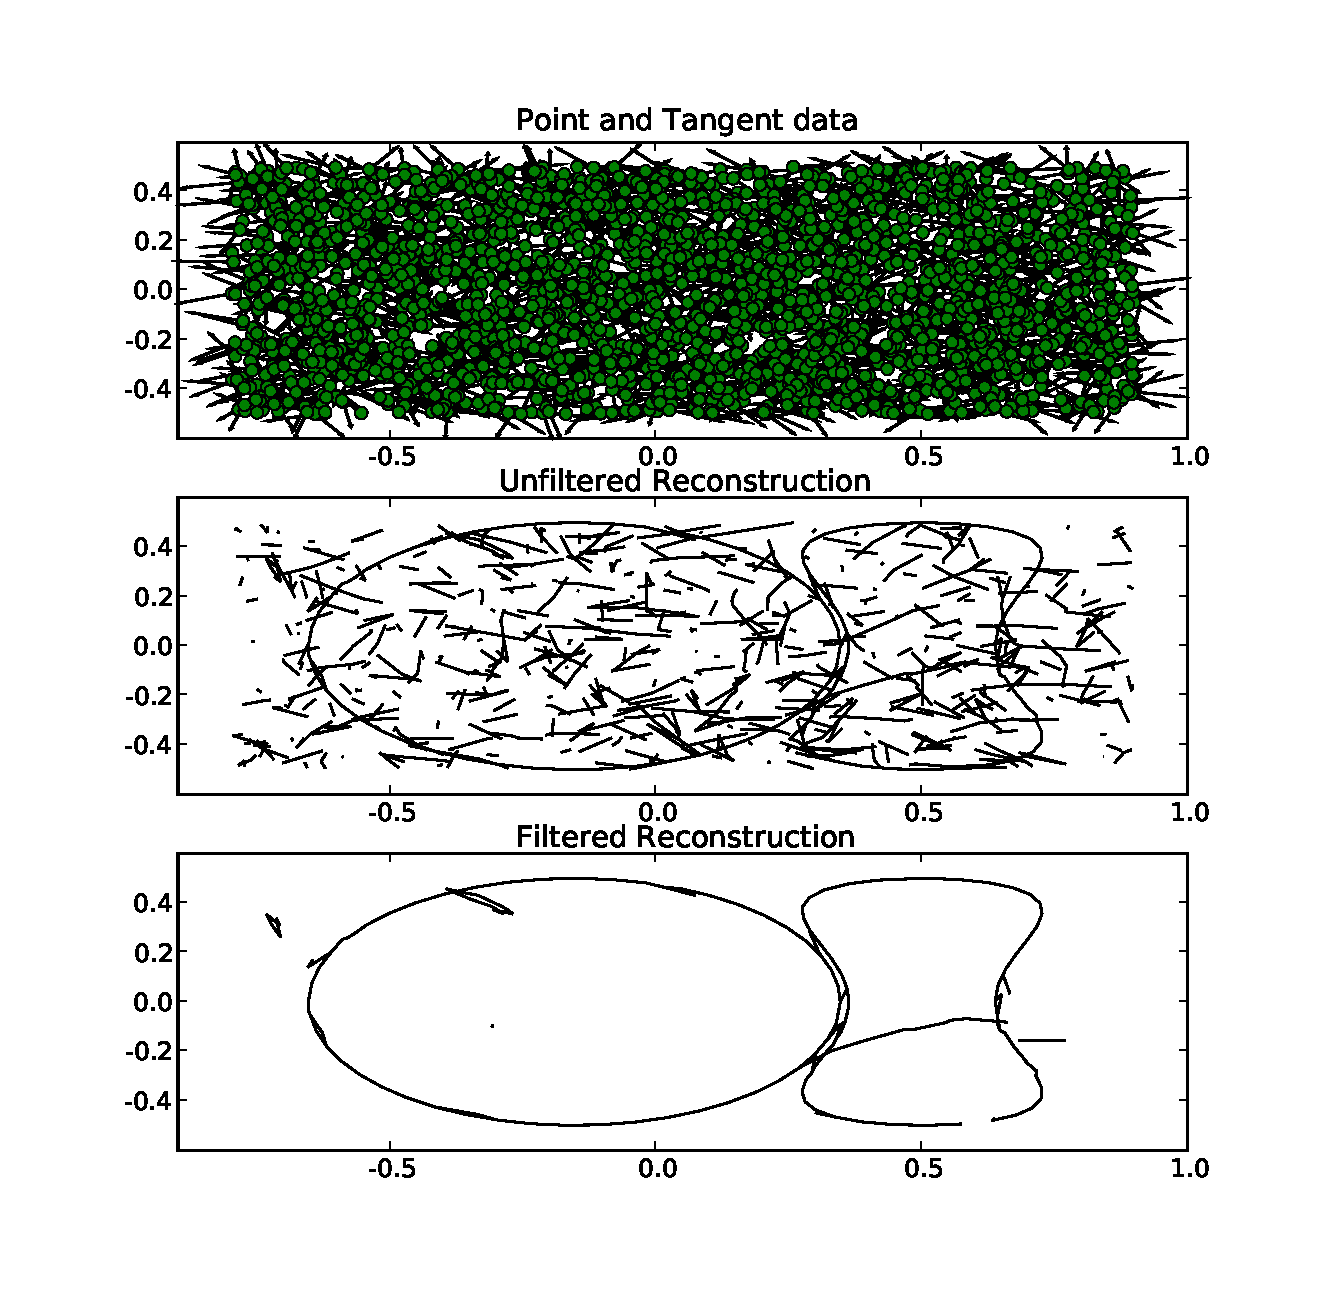
\includegraphics[scale=0.5]{more_noisy_example.eps}

\caption{The same example as in Figure \ref{fig:basicExample}, but with 2000 additional random points added (for a total of 2096). The original curve is no longer completely reconstructed, but the general shape is still roughly visible, along with many more spurious points. Filtering leaves with $l=4$ improves the situation considerably.}
\label{fig:moreNoisyExample}
\end{figure}

\appendix

\section{Speeding it up: an $O(N \log N)$ algorithm}
\label{sec:quadTreeSection}

As remarked earlier, Algorithm \ref{algo:polygonalization} runs in $O(N^{2})$ time as written. This can be remedied by using a spatially adaptive data structure. We propose the following data structure, which encapsulates naturally the geometry of our algorithm. We store the point/tangent pairs, $(\vp_{i},\vm_{i})$ in a quad-tree (sorted by $\vp_{i}$) which extends down to the scale $\min\{ \curvesep / 4, \curvemaxi / \sqrt{2} \}$. Making this scale smaller than $\delta$ is done to ensure that leaves can intersect only a single curve $\gamma$ in the figure $\curveSet$.

If a node of the tree at this scale has multiple points, we store them in a list which is sorted in the following way. We select a point at random on this node, call it $(\vp_{0},\vm_{0})$. The list is sorted according to the function $\vp_{i} \mapsto (\vp_{i} - \vp_{0}) \cdot \vm_{0}$. By our choice of the leaf size, only points coming from a single curve $\gamma \in \curveSet$ are contained in this node. Now, recalling the argument used in the proof of Lemma \ref{lem:closestTangentPointInAllowedRegionIsCorrect}, we find that near $\vp_{0}$, $\gamma(t)$ admits a parameterization of the form $\gamma(t)=\vp_{0} + \vm_{0} t + f(t) \vm_{0}^{\perp}$. This implies that sorting according to the function $(\vp_{i} - \vp_{0}) \cdot \vm_{0}$ will sort points according to their position on the curve $\gamma(t)$. We chose for the scale of leaf nodes to be smaller than $\curvemaxi / \sqrt{2}$ in order for this local parameterization to be valid.

//EXPLAIN HOW TO USE DATA STRUCTURE TO SPEED UP ALGORITHM//

\bibliography{../stucchio}
\bibliographystyle{hplain}

\end{document}